\documentclass{beamer}

\usepackage[utf8]{inputenc}
\usepackage[T1]{fontenc}
\usepackage[polish]{babel}

\usetheme{Madrid}

\title{Efektywna reprezentacja słownika}
\subtitle{Zaawansowane Biblioteki Programistyczne}
\author{Piotr Marcol}
\date{31.03.2026}

\begin{document}

\frame{\titlepage}

%------------------------------------------------

\begin{frame}{Cel projektu}
    \begin{itemize}
        \item Reprezentacja dużego zbioru słów w sposób efektywny
        \item Szybkie sprawdzanie przynależności słowa do słownika
        \item Minimalizacja zużycia pamięci
        \item Możliwość dalszych rozszerzeń (np. podpowiedzi, autouzupełnianie)
    \end{itemize}
\end{frame}

%------------------------------------------------

\begin{frame}{Problem}
    \begin{itemize}
        \item Duże słowniki (setki tysięcy słów)
        \item Powtarzające się prefiksy
        \item Naiwne przechowywanie (np. lista) jest nieefektywne
        \item Potrzeba szybkiego wyszukiwania
    \end{itemize}
\end{frame}

%------------------------------------------------

\begin{frame}{Podejścia}
    \begin{itemize}
        \item Tablica / lista słów
              \begin{itemize}
                  \item prosta implementacja
                  \item wolne wyszukiwanie
              \end{itemize}

        \item Drzewo prefiksowe (Trie)
              \begin{itemize}
                  \item współdzielenie prefiksów
                  \item szybkie operacje
              \end{itemize}

        \item Minimalny automat deterministyczny (DAFSA)
              \begin{itemize}
                  \item minimalna liczba stanów dla danego zbioru słów
                  \item bardzo wysoka efektywność
              \end{itemize}
    \end{itemize}
\end{frame}

%------------------------------------------------

\begin{frame}{Drzewo prefiksowe (Trie)}
    \begin{itemize}
        \item Każda krawędź odpowiada literze
        \item Ścieżka od korzenia tworzy słowo
        \item Wspólne prefiksy są współdzielone

              \vspace{0.5cm}
              Przykład:
              \begin{itemize}
                  \item \texttt{interview}, \texttt{internet}, \texttt{internal}, \texttt{interval}
              \end{itemize}

        \item Wspólny prefiks: \texttt{inter}
        \item Rozgałęzienie po różnych sufiksach
    \end{itemize}
    \begin{center}
        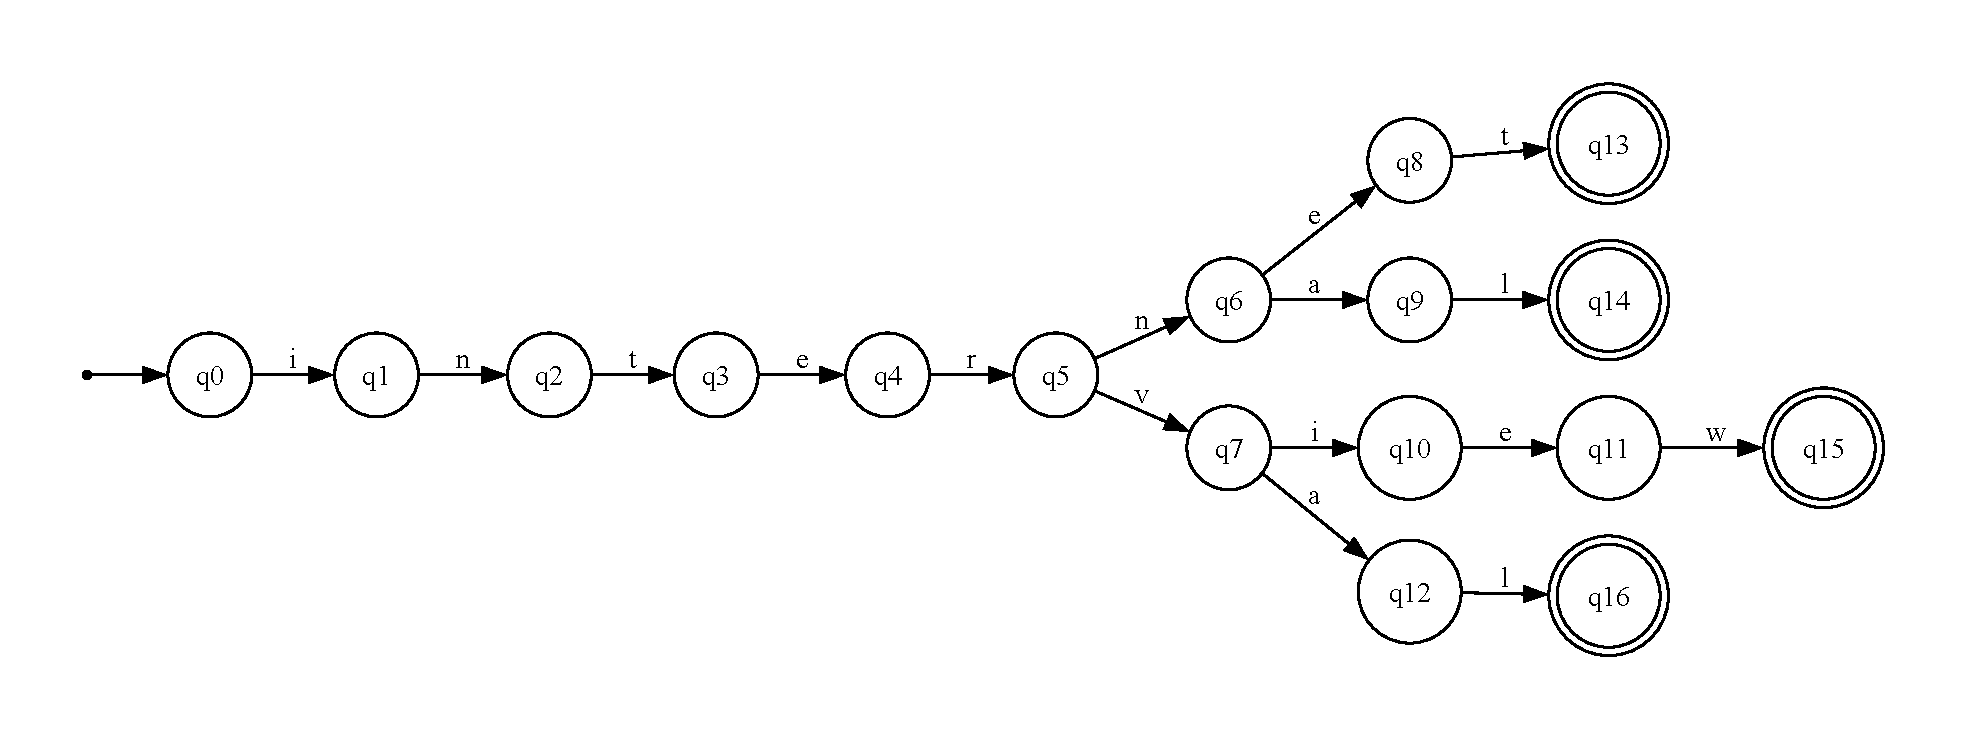
\includegraphics[width=\textwidth]{graphs/TRIE.pdf} % IGNORE
    \end{center}
\end{frame}

%------------------------------------------------

\begin{frame}{Stany akceptujące}
    \begin{itemize}
        \item Nie każdy węzeł oznacza słowo
        \item Węzły końcowe są oznaczane jako \textbf{akceptujące}

              \vspace{0.5cm}
              Przykład:
              \begin{itemize}
                  \item \texttt{banan} — stan akceptujący
                  \item \texttt{banana} — inny stan akceptujący
              \end{itemize}

        \item Jeden prefiks może być pełnym słowem i częścią innego
    \end{itemize}
    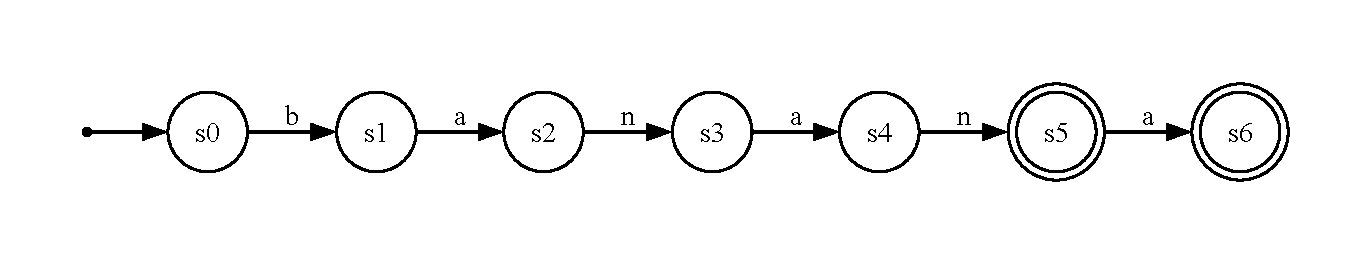
\includegraphics[width=\textwidth]{graphs/banan.pdf} % IGNORE
\end{frame}

%------------------------------------------------

\begin{frame}{Od Trie do automatu}
    \begin{itemize}
        \item Trie można traktować jako automat deterministyczny
        \item Każdy węzeł = stan
        \item Każda krawędź = przejście

              \vspace{0.5cm}
              Problem:
              \begin{itemize}
                  \item duża liczba stanów
              \end{itemize}

              Rozwiązanie:
              \begin{itemize}
                  \item minimalizacja automatu
              \end{itemize}
    \end{itemize}
\end{frame}

% ------------------------------------------------

\begin{frame}{Idea minimalizacji}
    \begin{itemize}
        \item Łączenie stanów o identycznych przejściach
        \item Identyczne sufiksy → jeden podgraf
        \item Proces od liści do korzenia

              \vspace{0.5cm}

        \item Efekt:
              \begin{itemize}
                  \item brak duplikacji końcówek
                  \item minimalna liczba stanów
              \end{itemize}
    \end{itemize}
\end{frame}

%------------------------------------------------

\begin{frame}{Minimalny automat (DAFSA)}
    % definicja DAFSA
    \begin{block}{Definicja}
        DAFSA to minimalny deterministyczny automat akceptujący skończony zbiór słów
    \end{block}
    \begin{itemize}
        \item Deterministyczny acykliczny automat skończony
        \item Łączy identyczne poddrzewa
        \item Eliminuje redundancję

              \vspace{0.5cm}
              Efekt:
              \begin{itemize}
                  \item mniej stanów
                  \item mniejsze zużycie pamięci
              \end{itemize}
    \end{itemize}
\end{frame}

% ------------------------------------------------

\begin{frame}{Ograniczenia}
    \begin{itemize}
        \item koszt budowy automatu
        \item trudniejsza implementacja niż Trie
        \item brak łatwej modyfikacji po zbudowaniu
    \end{itemize}
\end{frame}

%------------------------------------------------

\begin{frame}{Przykład optymalizacji}
    \begin{itemize}
        \item Słowa:
              \begin{itemize}
                  \item \texttt{running}
                  \item \texttt{walking}
              \end{itemize}

        \item Wspólny sufiks: \texttt{ing}

        \item W DAFSA:
              \begin{itemize}
                  \item końcówka \texttt{ing} przechowywana tylko raz
              \end{itemize}
    \end{itemize}
    \begin{center}
        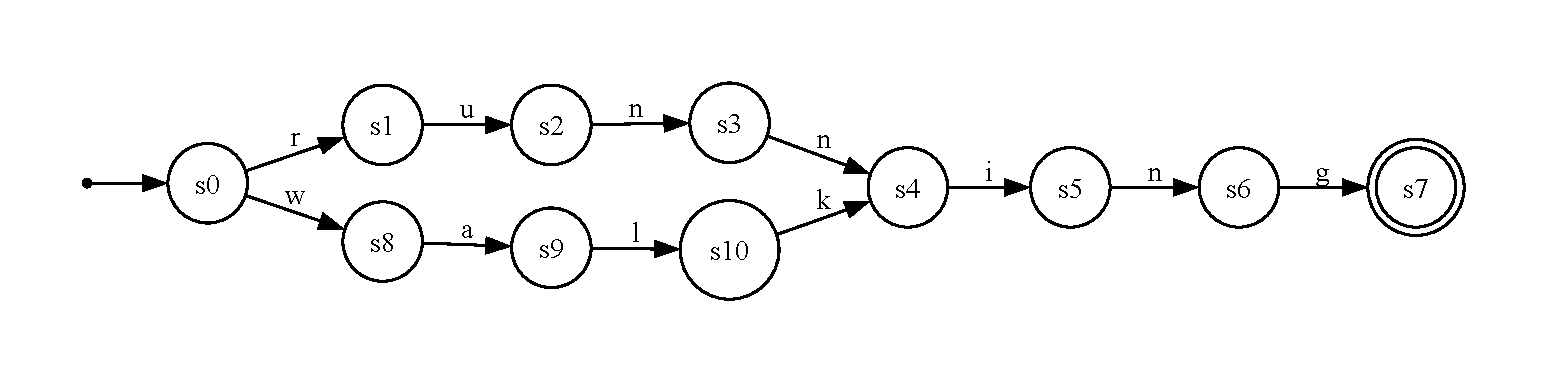
\includegraphics[width=\textwidth]{graphs/commonIng.pdf} % IGNORE
    \end{center}
\end{frame}

%------------------------------------------------

\begin{frame}{Przykład optymalizacji (cd.)}
    \begin{itemize}
        \item Słowa:
              \begin{itemize}
                  \item \texttt{interview}, \texttt{internet}, \texttt{internal}, \texttt{interval}
              \end{itemize}

        \item Wspólny prefiks: \texttt{inter}
        \item Wspólny sufiks: \texttt{al} dla \textit{internal} i \textit{interval}

        \item DAFSA łączy zarówno wspólne prefiksy, jak i sufiksy
    \end{itemize}
    \begin{center}
        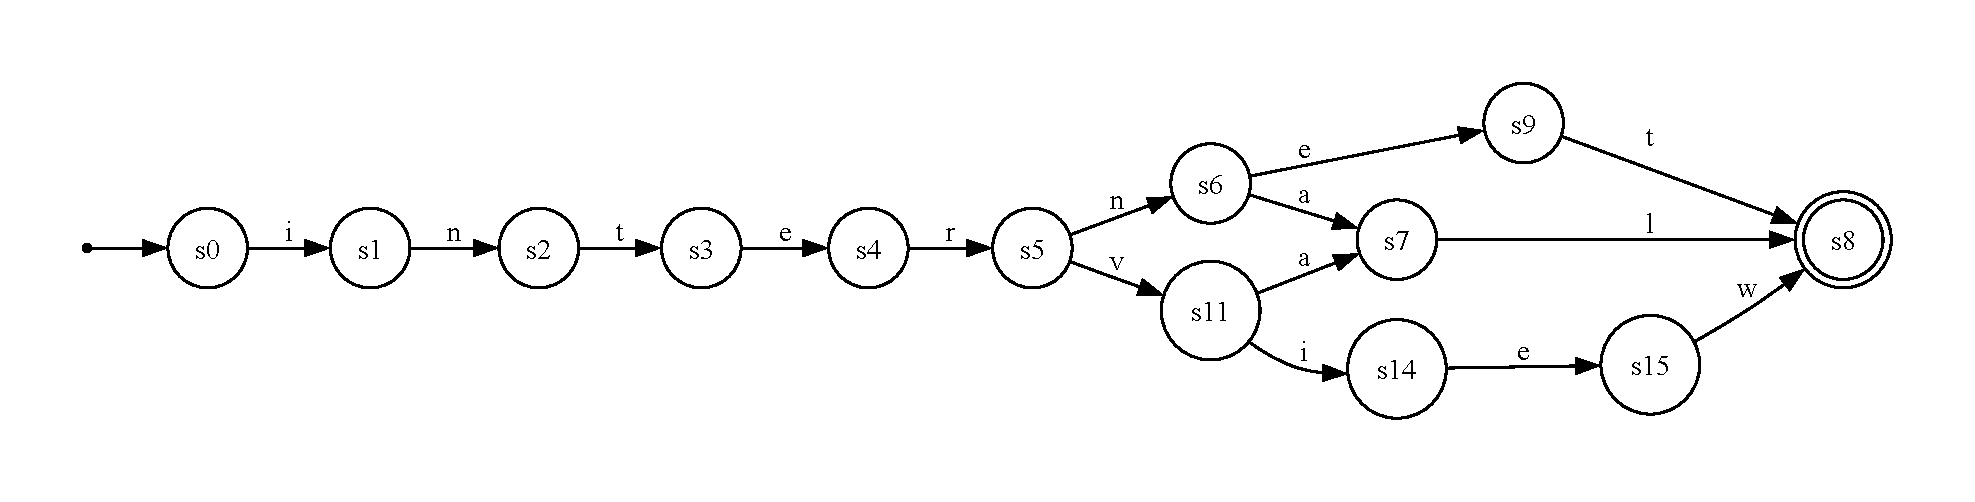
\includegraphics[width=\textwidth]{graphs/DAFSA.pdf} % IGNORE
    \end{center}
\end{frame}

%------------------------------------------------

\begin{frame}{Przykład optymalizacji (cd. 2)}
    \begin{itemize}
        \item Słowa: \texttt{kasa}, \texttt{kata}, \texttt{kosa}, \texttt{kota}

        \item Trie (12 stanów, 11 krawędzi):
              \begin{center}
                  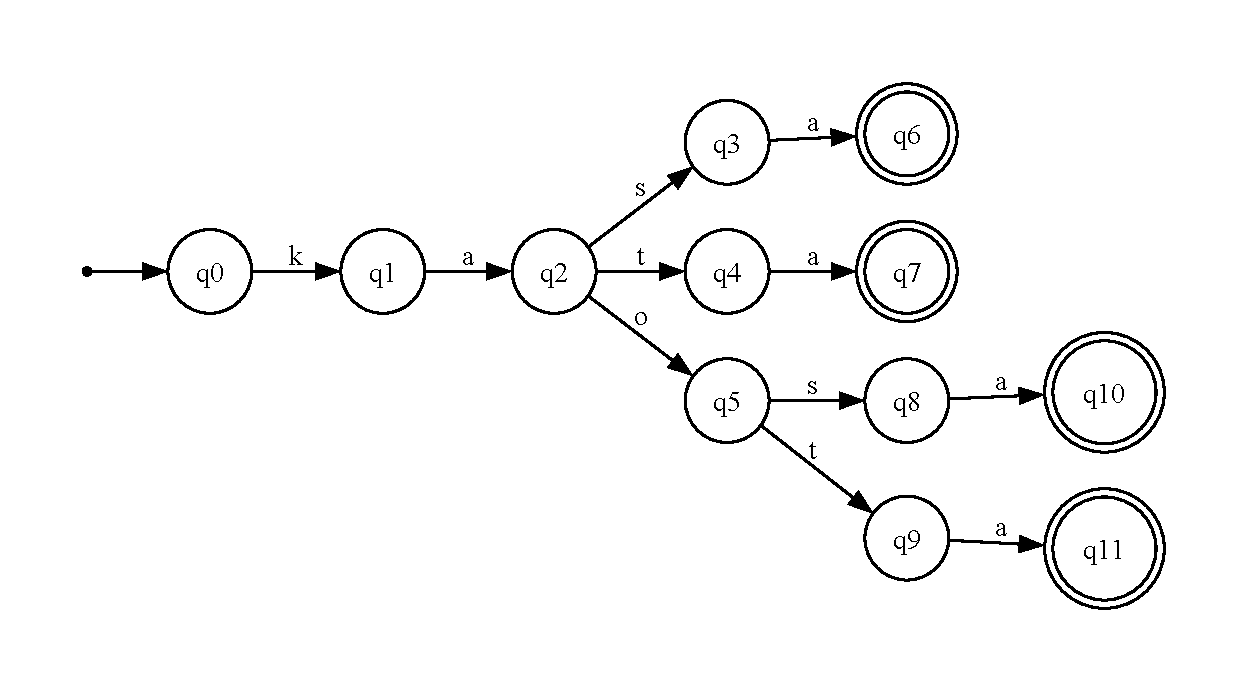
\includegraphics[width=0.6\textwidth]{graphs/kasa_trie.pdf} % IGNORE
              \end{center}

        \item Po minimalizacji (5 stanów, 6 krawędzi):
              \begin{center}
                  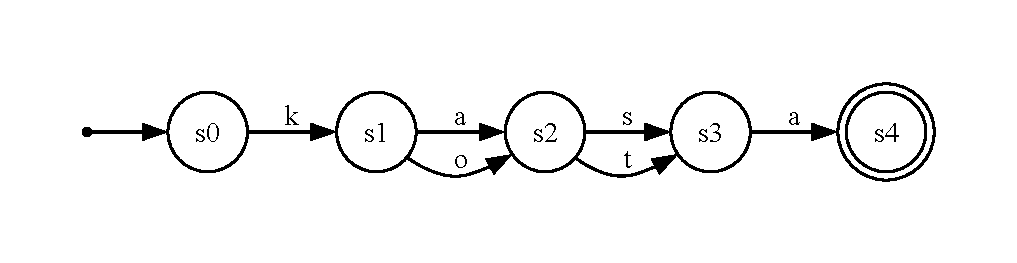
\includegraphics[width=0.8\textwidth]{graphs/kasa.pdf} % IGNORE
              \end{center}

    \end{itemize}
\end{frame}

% ------------------------------------------------

\begin{frame}{Trie vs DAFSA}
    \begin{itemize}
        \item \textbf{Trie}
              \begin{itemize}
                  \item optymalizuje wspólne prefiksy
                  \item prostsza implementacja
              \end{itemize}

        \item \textbf{DAFSA}
              \begin{itemize}
                  \item optymalizuje prefiksy i sufiksy
                  \item minimalna liczba stanów
              \end{itemize}

              \vspace{0.5cm}

        \item Najlepsze wyniki:
              \begin{itemize}
                  \item dane z powtarzalnymi fragmentami (prefiksy i/lub sufiksy)
              \end{itemize}
    \end{itemize}
\end{frame}

% ------------------------------------------------

\begin{frame}{Złożoność}
    \begin{itemize}
        \item Wyszukiwanie: O(m)
        \item Budowa:
              \begin{itemize}
                  \item Trie: O(sumy długości słów)
                  \item DAFSA: dodatkowy koszt minimalizacji
              \end{itemize}

        \item Pamięć:
              \begin{itemize}
                  \item Trie: większa
                  \item DAFSA: znacznie mniejsza
              \end{itemize}
    \end{itemize}
\end{frame}

% ------------------------------------------------

\begin{frame}{Dlaczego nie lista słów?}
    \begin{itemize}
        \item Lista:
              \begin{itemize}
                  \item wyszukiwanie: O($n \times m$)
                  \item duża redundancja danych
              \end{itemize}

        \item Trie / DAFSA:
              \begin{itemize}
                  \item wyszukiwanie: O(m)
                  \item współdzielenie struktur
                  \item oszczędność pamięci
              \end{itemize}
    \end{itemize}
\end{frame}

%------------------------------------------------

\begin{frame}{Możliwości rozszerzenia}
    \begin{itemize}
        \item Autouzupełnianie
        \item Wyszukiwanie prefiksowe
        \item Spell-check
        \item Analiza językowa
        \item Kompresja słowników
    \end{itemize}
\end{frame}

%------------------------------------------------

\begin{frame}{Proponowana architektura}
    \begin{itemize}
        \item Budowa Trie ze zbioru słów
        \item Konwersja do minimalnego automatu
        \item Interfejs do zapytań:
              \begin{itemize}
                  \item sprawdzenie przynależności słowa
                  \item zapytania prefiksowe
              \end{itemize}
        \item Reprezentacja jako graf stanów
    \end{itemize}
\end{frame}

%------------------------------------------------

\begin{frame}{Implementacja}
    \begin{itemize}
        \item Biblioteka w języku C++
        \item Reprezentacja słownika jako minimalizowany automat deterministyczny
        \item Wejście:
              \begin{itemize}
                  \item posortowany zbiór słów (porządek leksykograficzny)
              \end{itemize}
        \item Budowa:
              \begin{itemize}
                  \item inkrementalne dodawanie słów
                  \item częściowa minimalizacja w trakcie budowy
                  \item finalizacja minimalizacji (\texttt{finish()})
              \end{itemize}
        \item Operacje:
              \begin{itemize}
                  \item sprawdzanie przynależności słowa
                  \item zapytania prefiksowe
              \end{itemize}
    \end{itemize}
\end{frame}

%------------------------------------------------

\begin{frame}{Podsumowanie}
    \begin{itemize}
        \item Trie — prostota i czytelność
        \item DAFSA — optymalność pamięciowa
        \item Automaty — formalne i wydajne podejście
        \item Możliwość zastosowań w NLP i systemach wyszukiwania
    \end{itemize}
\end{frame}

%------------------------------------------------

\begin{frame}{Zastosowania}
    \begin{itemize}
        \item słowniki i spell-checkery
        \item autouzupełnianie (autocomplete)
        \item systemy wyszukiwania
        \item kompresja danych tekstowych
    \end{itemize}
\end{frame}

%------------------------------------------------

\begin{frame}{Dalsze kroki}
    \begin{itemize}
        \item Implementacja struktury
        \item Testy na dużych zbiorach danych
        \item Analiza wydajności
        \item Wizualizacja automatu
    \end{itemize}
\end{frame}

\begin{frame}
    \begin{center}
        \Huge Dziękuję za uwagę!
    \end{center}
\end{frame}

\frame{\titlepage}

\end{document}